\documentclass[leqno]{article}
% Shared QBT/Soln pack preamble for resources.danieljsmith.org.
\usepackage{graphicx}
\usepackage{dsfont}
\usepackage{mathtools}
\usepackage{amssymb}
\usepackage{amsmath}
\usepackage{mleftright}
\usepackage{amsthm}
\usepackage{float}
\usepackage{ragged2e}
\usepackage{tensor}
\usepackage{fancyhdr}
\usepackage{empheq}
\usepackage[most]{tcolorbox}
\usepackage{enumitem}
\usepackage{dirtytalk}
\usepackage{marginnote}
\usepackage{microtype}
\usepackage[
  a4paper,
  left=0.8in,
  right=1in,
  top=1in,
  bottom=0.5in,
  headheight=14pt,
  headsep=0.4in
]{geometry}
\setlength{\parindent}{0cm}

% TikZ / PGFPlots
\usepackage{pgfplots}
\pgfplotsset{compat=1.18}
\usepgfplotslibrary{fillbetween, polar}
\usetikzlibrary{calc, positioning}
\usetikzlibrary{angles, quotes}
\usetikzlibrary{arrows.meta}
\usetikzlibrary{decorations.pathreplacing, decorations.markings}
\usetikzlibrary{patterns}
\usetikzlibrary{intersections}

% Links and contents. The contents follow the TMUA papers: compact entries,
% no dot leaders, and each question's mark total in grey after its label.
\usepackage{tocloft}
\tocloftpagestyle{fancy}
\setlength{\cftbeforesubsecskip}{2pt}
\setlength{\cftsubsecindent}{1.5em}
\setlength{\cftsubsecnumwidth}{0pt}
\renewcommand{\cftsubsecfont}{\small\color{black}}
\renewcommand{\cftsubsecpagefont}{\small\color{black}}
\renewcommand{\cftsubsecleader}{\hfill}
\usepackage[colorlinks=true,linkcolor=black,citecolor=magenta,urlcolor=black]{hyperref}%
\urlstyle{same}

% Pack macros
% \marks also adds its value to the current question's total in the .aux
% file, so the contents show each total from the second pass. The write
% happens at shipout, so a box typeset more than once counts once. The
% pack's mark total for the contents-page title is summed the same way.
\makeatletter
\newcount\djs@totalmarks
\newcommand{\djsAddMarks}[2]{%
  \global\advance\djs@totalmarks#2\relax
  \@ifundefined{djs@marks@#1}%
    {\expandafter\xdef\csname djs@marks@#1\endcsname{#2}}%
    {\expandafter\xdef\csname djs@marks@#1\endcsname
      {\the\numexpr\csname djs@marks@#1\endcsname+#2\relax}}}
\RenewDocumentCommand{\marks}{o m}{%
  \protected@write\@auxout{}{\string\djsAddMarks{\number\value{enumi}}{#2}}%
  \IfValueTF{#1}%
    {\marginnote{\raggedright\textbf{[#2]}}[#1]}%
    {\marginnote{\raggedright\textbf{[#2]}}}%
}
\makeatother

\newcommand{\vspacerule}[2]{%
  \par\vspace*{#1}%
  \noindent\hrulefill\par
  \vspace*{#2}%
}

\definecolor{scarlet}{RGB}{205, 40, 75}
% Site colours for the contents-page title: the accent, the rule colour, a
% stronger rule colour for the path separator, and the muted text colour.
\definecolor{djsBurgundy}{RGB}{118, 59, 67}
\definecolor{djsHairline}{RGB}{216, 213, 205}
\definecolor{djsSlash}{RGB}{170, 166, 158}
\definecolor{djsMuted}{RGB}{96, 101, 106}

% Worked-solution box, adapted from the TMUA worked-solutions box. A white breakable box with a left scarlet rule and no surrounding
% frame or tint. A part that breaks fills the rest of its page, so the rule
% runs to the bottom margin; the unbroken or last part ends in a short
% horizontal foot rule so a solution visibly stops. Unlike the TMUA box there
% is no answer label. The box does not grow to the left, so the rule sits at
% the text edge; growing to the right keeps the usable line width close to the
% old tcolorbox Solution box.
% Spacing inside the box: paragraphs are 6pt apart, so source blank lines show
% (solutions put one after each display and none between a lead-in and its
% display). Every display gets 6pt above and 10pt below, whatever the length
% of its lead-in line; align rows are spread by an 8pt \jot; solution parts
% are 14pt apart and sub-parts 8pt; \left and \right space like ordinary
% brackets (mleftright); no single line is stranded at a page break; and
% neither the Solution label nor the line before a list ends a page. No
% skip can shrink, so full pages are not squeezed.
\newtcolorbox{djsSolution}{%
  enhanced, breakable, frame hidden, sharp corners, colback=white,
  height fixed for=first and middle, height fill,
  extras unbroken and last={natural height},
  borderline west={2.2pt}{0pt}{scarlet},
  left=11pt, right=0pt, top=5pt, bottom=13pt,
  before skip=13pt, after skip=4pt,
  grow to right by=10mm,
  overlay unbroken and last={%
    \fill[scarlet] (frame.south west)
      rectangle ([xshift=3.5cm, yshift=2.2pt]frame.south west);},
  before upper={{\color{scarlet}\bfseries Solution}\par\nobreak\vspace{4pt}%
    \setlength{\parskip}{6pt plus 2pt}%
    \setlength{\abovedisplayskip}{6pt plus 2pt}%
    \setlength{\abovedisplayshortskip}{6pt plus 2pt}%
    \setlength{\belowdisplayskip}{10pt plus 2pt}%
    \setlength{\belowdisplayshortskip}{10pt plus 2pt}%
    \setlength{\jot}{8pt}%
    \setlist{parsep=6pt plus 2pt, topsep=6pt plus 2pt, beginpenalty=10000}%
    \setlist[enumerate,1]{itemsep=14pt plus 2pt}%
    \setlist[enumerate,2]{itemsep=8pt plus 2pt}%
    \mleftright
    \clubpenalty=10000 \widowpenalty=10000 \displaywidowpenalty=10000\relax}}

% Optional smaller figure inside a solution box. \scalebox shrinks node text
% with the drawing. Not applied to existing figures.
\newcommand{\SolnFigureScale}{0.85}
\newsavebox{\djsSolnFigureBox}
\newenvironment{djsSolutionFigure}
  {\par\vspace{4pt}\begin{center}\begin{lrbox}{\djsSolnFigureBox}}
  {\end{lrbox}\scalebox{\SolnFigureScale}{\usebox{\djsSolnFigureBox}}%
   \end{center}\vspace{2pt}\par}

\newcommand{\cxl}[2]{%
  \tikz[baseline=(X.base)]{%
    \node[inner sep=0pt, outer sep=0pt, text=#1] (X) {$#2$};
    \draw[#1, line width=0.4pt] (X.south west)--(X.north east);
  }%
}

% Page-style hook run at the contents page and each question's opening page.
% A no-op for QBT packs; \djsSolnHeader points it at the fancy header.
\newcommand{\djsQuestionPageStyle}{}

% A contents entry: "Question N" in a box wide enough for two digits, so the
% mark totals line up, then the total in grey. Bookmarks keep "Question N".
\makeatletter
\newlength{\djsTocLabelWidth}
\newcommand{\djsTocMarks}[1]{%
  \@ifundefined{djs@marks@#1}{}{%
    {\footnotesize\itshape\color{black!45}%
     \csname djs@marks@#1\endcsname~mark%
     \ifnum\csname djs@marks@#1\endcsname=1 \else s\fi}}}
\newcommand{\djsTocEntry}[1]{%
  \texorpdfstring
    {\settowidth{\djsTocLabelWidth}{Question 00}%
     \makebox[\dimexpr\djsTocLabelWidth+0.9em\relax][l]{Question #1}%
     \djsTocMarks{#1}}%
    {Question #1}}
\makeatother

% The question count for the contents-page title is written to the .aux at
% the end of the document, so it also appears from the second pass.
\newcounter{djsQuestions}
\newcommand{\questionitem}{%
  \djsQuestionPageStyle
  \item\phantomsection
  \stepcounter{djsQuestions}%
  \addcontentsline{toc}{subsection}{\protect\djsTocEntry{\number\value{enumi}}}%
}
\makeatletter
\newcommand{\djsSetQuestionCount}[1]{\gdef\djs@questioncount{#1}}
\AtEndDocument{\immediate\write\@auxout
  {\string\djsSetQuestionCount{\number\value{djsQuestions}}}}
\makeatother

\renewcommand{\contentsname}{Questions}

% \djsPackHeader[<link content tag>]{<left header>}; the tag says which
% document a click on the header link came from.
\newcommand{\djsPackHeader}[2][questions]{%
  \pagestyle{fancy}%
  \fancyhead{}%
  \fancyfoot{}%
  \renewcommand{\headrulewidth}{0.9pt}%
  \lhead{#2}%
  \chead{}%
  \rhead{\href{https://danieljsmith.org/?utm_source=pdf&utm_campaign=further-maths&utm_content=#1}{danieljsmith.org}}%
}

% The header's topic is also the contents-page title, under which a label
% says which booklet this is.
\newcommand{\djsPackTitle}{}
\newcommand{\djsBookletLabel}{}
\newcommand{\djsQbtHeader}[1]{%
  \djsPackHeader{#1}%
  \renewcommand{\djsPackTitle}{#1}%
  \renewcommand{\djsBookletLabel}{Questions by topic}%
}

% The colophon at the foot of page one, independent of the page style: the
% contents-page title's hairline led by a short scarlet rule, then the date on
% the left and a link to the site on the right, all inside the bottom margin.
% Its sizes are fixed, so it matches the TMUA papers' colophon. The document
% supplies the date; recompiling never changes it.
\makeatletter
\newcommand{\djsLastUpdated}[1]{%
  \AtBeginDocument{\AddToHookNext{shipout/foreground}{\djs@colophon{#1}}}}
\newcommand{\djs@colophon}[1]{%
  \put(0.8in,-\dimexpr\paperheight-0.47in\relax){%
    \makebox[0pt][l]{\color{djsHairline}%
      \rule[0.9pt]{\dimexpr\paperwidth-1.8in\relax}{0.6pt}}%
    \makebox[0pt][l]{\color{scarlet}\rule{3.5cm}{2.2pt}}}%
  \put(0.8in,-\dimexpr\paperheight-0.32in\relax){\makebox[0pt][l]{%
    \fontsize{9}{11}\selectfont Last updated #1}}%
  \put(\dimexpr\paperwidth-1in\relax,-\dimexpr\paperheight-0.32in\relax){%
    \makebox[0pt][r]{\fontsize{7}{8.5}\selectfont\color{djsMuted}%
      Latest version at \href{https://resources.danieljsmith.org/}%
        {\color{black}resources.danieljsmith.org}}}}
\makeatother

% Solutions packs show the header only on the contents page and each
% question's opening page, so it never appears part-way through a solution.
% \thispagestyle marks the next page shipped out, which is the question's
% page because every solution question starts after a \newpage.
\newcommand{\djsSolnHeader}[1]{%
  \djsPackHeader[solutions]{\textit{Solutions} - #1}%
  \pagestyle{empty}%
  \renewcommand{\djsQuestionPageStyle}{\thispagestyle{fancy}}%
  \renewcommand{\djsPackTitle}{#1}%
  \renewcommand{\djsBookletLabel}{Worked solutions}%
}

% \djsSitePath{<strand>}{<topic>}, called once after the header, names where
% the pack sits on the site; the contents-page title prints it above the pack
% title, e.g. CORE PURE / FURTHER CALCULUS. Without it the line is left out.
\makeatletter
\newif\ifdjs@sitepath
\newcommand{\djs@strand}{}
\newcommand{\djs@section}{}
\newcommand{\djsSitePath}[2]{%
  \djs@sitepathtrue
  \renewcommand{\djs@strand}{#1}%
  \renewcommand{\djs@section}{#2}%
}
\makeatother

% Further Mechanics packs call \djsMechanicsPack in their preamble, so that
% \djsFrontMatter prints the default value of g above the contents. The box
% keeps its own space above it (before skip is the whole gap below the title,
% not an addition to it). Without the box, \djsGravityNote is just extra space
% before the contents heading, bringing the gap above it close to the gap
% between the box and the heading on Further Mechanics pages.
\newcommand{\djsGravityNote}{\vspace{14pt}}
\newcommand{\djsMechanicsPack}{%
  \renewcommand{\djsGravityNote}{%
    \begin{tcolorbox}[sharp corners, colback=white, colframe=black,
      boxrule=1pt, left=8pt, right=8pt, top=6pt, bottom=6pt,
      before skip=20pt]
    {\bfseries Instructions}\par\vspace{4pt}
    Unless a question states otherwise, take $g = 9.8\,\mathrm{m\,s^{-2}}$
    wherever a numerical value of $g$ is required. Solutions also give final
    answers for $g = 10\,\mathrm{m\,s^{-2}}$ where these differ.
    \end{tcolorbox}%
    \vspace{16pt}}%
}

% Contents-page title: the site path in spaced burgundy capitals, the pack
% title, a hairline led by a short scarlet rule (the solution box's foot rule),
% then the booklet label with the question and mark counts. The counts come
% from the .aux, so they appear from the second pass.
\makeatletter
\newsavebox{\djs@eyebrowbox}
\newcommand{\djs@caps}[1]{\textls[180]{\MakeUppercase{#1}}}
\newcommand{\djs@eyebrow}{%
  \color{djsBurgundy}\footnotesize\bfseries
  \djs@caps{\djs@strand}%
  {\color{djsSlash}\hspace{0.55em}/\hspace{0.55em}}%
  \djs@caps{\djs@section}}
\newcommand{\djs@dot}{\hspace{0.45em}\textperiodcentered\hspace{0.45em}}
\newcommand{\djs@counts}{%
  \@ifundefined{djs@questioncount}{}{%
    \djs@questioncount~question\ifnum\djs@questioncount=1 \else s\fi
    \ifnum\djs@totalmarks>0
      \djs@dot\the\djs@totalmarks~mark\ifnum\djs@totalmarks=1 \else s\fi
    \fi}}
\newcommand{\djsContentsTitle}{%
  \ifdjs@sitepath
    \sbox\djs@eyebrowbox{\djs@eyebrow}%
    \ifdim\wd\djs@eyebrowbox>\linewidth
      \@latex@warning@no@line{The \string\djsSitePath\space line is wider
        than the text, so it wraps. Shorten its topic}%
    \fi
    {\raggedright\djs@eyebrow\par}%
    \vspace{7pt}%
  \fi
  {\raggedright\fontsize{24.88}{28}\selectfont\djsPackTitle\par}%
  \vspace{9pt}%
  \noindent\makebox[0pt][l]{\color{djsHairline}\rule[0.9pt]{\linewidth}{0.6pt}}%
  {\color{scarlet}\rule{3.5cm}{2.2pt}}\par
  \vspace{5pt}%
  {\small\color{djsMuted}\djsBookletLabel\hfill\djs@counts\par}%
  \vspace{8pt}%
}
\makeatother

\newcommand{\djsFrontMatter}{%
  \djsQuestionPageStyle
  \vspace*{6pt}%
  \djsContentsTitle
  \djsGravityNote
  \tableofcontents
  \newpage
}


\djsQbtHeader{Polar Coordinates Basics}
\djsSitePath{Core Pure}{Polar Coordinates}
\djsLastUpdated{13 October 2026}

\begin{document}
\djsFrontMatter
\begin{enumerate}[
  label=\textbf{\arabic*.},
  leftmargin=*,
  topsep=0pt,
  partopsep=0pt,
  parsep=0pt
]

% ---- Question 1 ----
\questionitem
% [Source: _QBT__Polar_Coordinates_Basics, Q1]

\begin{figure}[H]
    \centering
\begin{tikzpicture}[scale=1.5]
\def\displayunit{0.35}
\def\rstart{1}
\def\growth{2}
\def\outerradius{8}
\pgfmathsetmacro{\tmax}{pi}
\pgfmathsetmacro{\endpoint}{\displayunit*(\rstart+\growth*\tmax)}
\pgfmathsetmacro{\axisend}{1.2*\displayunit*\outerradius}
\pgfmathsetmacro{\workspace}{1.15*\displayunit*\outerradius}
\coordinate (O) at (0,0);
\coordinate (A) at (180:\endpoint);
\coordinate (L) at (\axisend,0);
\path[use as bounding box] (-\workspace,-\workspace) rectangle (\axisend,\workspace);
\draw[thick, black, samples=200, domain=0:\tmax, variable=\t]
  plot ({\displayunit*(\rstart+\growth*\t)*cos(deg(\t))},{\displayunit*(\rstart+\growth*\t)*sin(deg(\t))});
\draw[-{Stealth[length=3mm]}, thick, black] (O) -- (L);
\fill[black] (O) circle (1.5pt);
\node[below left=2pt] at (O) {$O$};
\node[left=2pt] at (A) {$A$};
\node[below] at (L) {Initial line};
\end{tikzpicture}
\end{figure}


The polar curves $C_1$ and $C_2$ are defined by
\[
C_1: r=1+2\theta,\qquad 0\leqslant\theta\leqslant\pi
\] \\
and
\[
C_2: r=8-\theta,\qquad 0\leqslant\theta\leqslant2\pi
\] \\
The diagram above shows $C_1$. Its endpoint $A$ lies on the ray opposite the initial line. \\
\begin{enumerate}[label=\textbf{(\alph*)}]
\item State the polar coordinates of $A$ and find its Cartesian coordinates, taking the pole as the origin and the initial line as the positive $x$-axis. \marks{3} \\
\item Find the polar coordinates of the point where $C_1$ and $C_2$ intersect. \marks{2} \\
\item On a copy of the diagram above, sketch $C_2$, indicating the radii of its two endpoints. \marks{1} \\
\end{enumerate}

\newpage

% ---- Question 2 ----
\questionitem
% [Source: _QBT__Polar_Coordinates_Basics, Q2]

The curve $C$ has the polar equation
\[
r=\frac{6}{2-\sin\theta},\qquad -\pi<\theta\leq\pi
\] \\
\begin{enumerate}[label=\textbf{(\alph*)}]
\item Verify that the point with polar coordinates $\left(4,\dfrac{\pi}{6}\right)$ lies on $C$. \marks{1} \\
\item Find the exact polar coordinates of the point on $C$ which is furthest from the pole, $O$. \marks{3} \\
\item The Cartesian line $y=x$ intersects $C$ at two points. Find the exact Cartesian coordinates of both points. \marks{4} \\
\end{enumerate}

\newpage

% ---- Question 3 ----
\questionitem
% [Source: _QBT__Polar_Coordinates_Basics, Q3]

\begin{figure}[H]
    \centering
\begin{tikzpicture}[scale=1.5, x=0.65cm, y=0.65cm]
\def\base{4}
\def\amp{3}
\def\axislen{2.5}
\def\leftspace{7.5}
\def\rightspace{3.5}
\def\verticalspace{5.3}
\coordinate (O) at (0,0);
\coordinate (InitialEnd) at (\axislen,0);
\path[use as bounding box] (-\leftspace,-\verticalspace) rectangle (\rightspace,\verticalspace);
\draw[thick, black, domain=0:180, samples=200, variable=\t]
  plot ({(\base-\amp*cos(\t))*cos(\t)},{(\base-\amp*cos(\t))*sin(\t)});
\draw[-{Stealth[length=3mm]}, thick, black] (O) -- (InitialEnd)
  node[right] {$\theta=0$};
\node[left] at (O) {$O$};
\end{tikzpicture}
\end{figure}


The curve $C$ has polar equation
\[
r=4-3\cos\theta,\qquad -\pi<\theta\leq\pi
\] \\
\begin{enumerate}[label=\textbf{(\alph*)}]
\item The diagram above shows the portion of $C$ for which $0\leq\theta\leq\pi$. Complete the sketch of $C$. \marks{1} \\
\end{enumerate}
The straight line $\ell$ has polar equation
\[
r\cos\theta=1
\] \\
\begin{enumerate}[label=\textbf{(\alph*)}, resume]
\item Add $\ell$ to your completed sketch and find all the points of intersection of $C$ and $\ell$. Give their polar coordinates, with radii exact and any non-zero angles in radians to $3$ significant figures. \marks{6} \\
\end{enumerate}

\newpage

% ---- Question 4 ----
\questionitem
% [Source: _QBT__Polar_Coordinates_Basics, Q4]

The curve $C_1$ has polar equation
\[
r^2+4r\cos\theta-6r\sin\theta=12
\] \\
where $r>0$ and $-\pi<\theta\leq\pi$. \\
\begin{enumerate}[label=\textbf{(\alph*)}]
\item Find a Cartesian equation for $C_1$ and show that it represents a circle. State its radius and the Cartesian coordinates of its centre. \marks{4} \\
\item Sketch $C_1$, marking its centre and the pole. Find the exact greatest and least distances of a point on $C_1$ from the pole. \marks{4} \\
\end{enumerate}

\newpage

% ---- Question 5 ----
\questionitem
% [Source: _QBT__Polar_Coordinates_Basics, Q5]

\begin{enumerate}[label=\textbf{(\alph*)}]
\item The curve $C_1$ has Cartesian equation
\[
x^2+y^2=\sqrt{3}\,y
\] \\
Find the centre and radius of $C_1$, and show that its non-pole points have polar equation $r=\sqrt{3}\sin\theta$. \marks{4} \\
\end{enumerate}
The curve $C_2$ has polar equation
\[
r=1+\cos\theta
\] \\
Consider both curves for $0<\theta<\pi$, together with their limiting endpoints. \\
In this interval, $r>0$ for both curves. The pole is a limiting endpoint of each curve. \\
\begin{enumerate}[label=\textbf{(\alph*)}, resume]
\item Show that $C_1$ and $C_2$ have exactly one intersection other than the pole, and find the exact polar coordinates of this intersection, $P$. \marks{4} \\
\item Sketch both curves on a single diagram, clearly labelling each curve. Mark $P$ and indicate the Cartesian coordinates of every point where either curve meets the initial line. \marks{3} \\
\end{enumerate}

\newpage

% ---- Question 6 ----
\questionitem
% [Source: _QBT__Polar_Coordinates_Basics, Q6]

A curve has Cartesian equation
\[
(x^2+y^2)^2=5x^2+4xy+2y^2
\] \\
where $x$ and $y$ are not both zero. Use the convention $r>0$. \\
\begin{enumerate}[label=\textbf{(\roman*)}]
\item Show that the polar equation of the curve is
\[
r^2=\frac{7+3\cos 2\theta+4\sin 2\theta}{2}
\] \marks[-30pt]{4}
\item Hence find the least and greatest distances of points on the curve from the origin, giving your answers in exact form. \marks{3} \\
\end{enumerate}

\newpage

% ---- Question 7 ----
\questionitem
% [Source: _QBT__Polar_Coordinates_Basics, Q7]

\begin{figure}[H]
    \centering
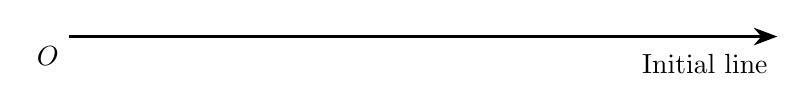
\begin{tikzpicture}[scale=1.5]
\def\raylen{6}
\coordinate (O) at (0,0);
\coordinate (E) at ($(O)+(\raylen,0)$);
\draw[thick, black, -{Stealth[length=3mm]}] (O) -- (E);
\node[below left] at (O) {$O$};
\node[below left, yshift=-3pt] at (E) {Initial line};
\end{tikzpicture}
\end{figure}


The graph $G_1$ has polar equation
\[
r=6\sec\left(\theta+\frac{\pi}{6}\right),\qquad -\frac{2\pi}{3}<\theta<\frac{\pi}{3}
\] \\
The graph $G_2$ is the ray with polar equation
\[
\theta=-\alpha,\qquad r>0
\] \\
where $0<\alpha<\dfrac{\pi}{2}$. \\
\begin{enumerate}[label=\textbf{(\alph*)}]
\item Show that $G_1$ is a straight line by finding its Cartesian equation in the form $y=mx+c$. \marks{3} \\
\item On a copy of the diagram above, sketch $G_1$ and $G_2$. Label the angle $\alpha$ and give the polar coordinates of the intersection of $G_1$ with the initial line. \marks{3} \\
\item Find, in terms of $\alpha$, the polar coordinates of the intersection of $G_1$ and $G_2$. \marks{2} \\
\item The region bounded by the initial line, $G_1$ and $G_2$ has area $12\sqrt{3}$ square units. Determine the exact value of $\alpha$. \marks{4} \\
\end{enumerate}

\newpage

% ---- Question 8 ----
\questionitem
% [Source: _QBT__Polar_Coordinates_Basics, Q8]

\begin{figure}[H]
    \centering
\begin{tikzpicture}[scale=1.5]
\def\radScale{2}
\def\frequency{3}
\pgfmathsetmacro{\alphaDraw}{180/\frequency}
\pgfmathsetmacro{\rayLength}{\radScale}
\pgfmathsetmacro{\axisLength}{2.3*\radScale}
\coordinate (O) at (0,0);
\coordinate (T) at (\alphaDraw:\rayLength);
\coordinate (H) at (\axisLength,0);
\draw[thick, black, domain=0:\alphaDraw, samples=180, variable=\t]
  plot ({\radScale*(1+cos(\frequency*\t))*cos(\t)},{\radScale*(1+cos(\frequency*\t))*sin(\t)});
\draw[thick, black, -{Stealth[length=3mm]}] (O) -- (H);
\draw[dashed, black] (O) -- (T);
\node[below left] at (O) {$O$};
\node[right] at (H) {$\theta=0$};
\node[above right] at (T) {$\theta=\alpha$};
\end{tikzpicture}
\end{figure}


A curve has polar equation
\[
r=2(1+\cos 3\theta),\qquad 0\leq\theta<2\pi
\] \\
with only points for which $r>0$ represented by polar coordinates. The pole $O$ is included as a limiting point of the curve. \\
\begin{enumerate}[label=\textbf{(\roman*)}]
\item The diagram above shows the arc traced from $\theta=0$ until the curve first reaches $O$. The tangent there has equation $\theta=\alpha$, where $0<\alpha<\pi$. Find $\alpha$ in terms of $\pi$. \marks{2} \\
\item
\begin{enumerate}[label=(\alph*)]
\item Let $f(\theta)=2(1+\cos 3\theta)$. Show that, for every integer $k$,
\[
f\left(\frac{2k\pi}{3}-\theta\right)=f(\theta)
\] \\
and also show that
\[
f\left(\theta+\frac{2\pi}{3}\right)=f(\theta)
\] \marks[-30pt]{4}
\item Hence state the equations of all the distinct lines of symmetry of the curve, using angles in $0\leq\theta<\pi$. State also the smallest positive angle through which the curve can be rotated about $O$ and remain unchanged. \marks{3} \\
\end{enumerate}
\item Sketch the complete curve. State its maximum radius and all the corresponding values of $\theta$ in $0\leq\theta<2\pi$. \marks{4} \\
\end{enumerate}

\newpage

% ---- Question 9 ----
\questionitem
% [Source: _QBT__Polar_Coordinates_Basics, Q9]

\begin{enumerate}[label=\textbf{(\alph*)}]
\item The line $L$ has polar equation
\[
r=3\sec\left(\theta-\frac{\pi}{4}\right),\qquad -\frac{\pi}{4}<\theta<\frac{3\pi}{4}
\] \\
Show that its Cartesian equation is $x+y=3\sqrt{2}$. \marks{2} \\
\item The curve $C$ has polar equation
\[
r=5-2\sin 2\theta,\qquad -\pi<\theta\leq\pi
\] \\
Find the exact polar coordinates of all the points of intersection of $L$ and $C$. \\
Fully justify that you have found every point of intersection. \marks{6} \\
\end{enumerate}

\newpage

% ---- Question 10 ----
\questionitem
% [Source: _QBT__Polar_Coordinates_Basics, Q10]

\begin{enumerate}[label=\textbf{(\alph*)}]
\item The curve $C$ is the right-hand branch of the hyperbola
\[
x^2-y^2=6x,\qquad x\geq6
\] \\
Using $x=r\cos\theta$ and $y=r\sin\theta$, show that its polar equation is
\[
r=6\cos\theta\sec 2\theta,\qquad -\frac{\pi}{4}<\theta<\frac{\pi}{4}
\] \\
where $r>0$. \marks{3} \\

\begin{figure}[H]
    \centering
\begin{tikzpicture}[scale=0.4]
\def\xmax{17}
\def\ymax{12}
\def\ymin{-12}
\def\coef{6}
\pgfmathsetmacro{\halfcoef}{\coef/2}
\coordinate (O) at (0,0);
\coordinate (E) at (\xmax,0);
\begin{scope}
  \clip (0,\ymin) rectangle (\xmax,\ymax);
  \draw[thick, black, samples=200, domain=\ymin:\ymax, variable=\u]
    plot ({\halfcoef+sqrt(\halfcoef*\halfcoef+\u*\u)},{\u});
\end{scope}
\draw[-{Stealth[length=3mm]}, thick, black] (O) -- (E);
\node[below left] at (O) {$O$};
\node[below] at ($(O)!0.75!(E)$) {Initial line};
\end{tikzpicture}
\end{figure}


\item The diagram above shows the curve $C$. \\
\begin{enumerate}[label=(\roman*)]
\item Find the polar coordinates of the point $N$ on $C$ nearest to the pole $O$. Justify that your point gives the minimum value of $r$. \marks{3} \\
\item The circle $r=6\sqrt{3}$ meets $C$ at $P$ and $Q$, where $P$ lies above the initial line and $Q$ lies below it. Find their exact polar coordinates, using angles in the interval $-\dfrac{\pi}{4}<\theta<\dfrac{\pi}{4}$. \marks{5} \\
\item Find the exact value, in radians, of the angle $PNQ$. \marks{4} \\
\end{enumerate}
\end{enumerate}

\end{enumerate}
\end{document}
